% Created 2021-07-16 Fri 01:07
% Intended LaTeX compiler: pdflatex
\documentclass[11pt]{article}
\usepackage[utf8]{inputenc}
\usepackage[T1]{fontenc}
\usepackage{graphicx}
\usepackage{grffile}
\usepackage{longtable}
\usepackage{wrapfig}
\usepackage{rotating}
\usepackage[normalem]{ulem}
\usepackage{amsmath}
\usepackage{textcomp}
\usepackage{amssymb}
\usepackage{capt-of}
\usepackage{hyperref}
\date{\today}
\title{}
\hypersetup{
 pdfauthor={},
 pdftitle={},
 pdfkeywords={},
 pdfsubject={},
 pdfcreator={Emacs 27.2 (Org mode 9.4.4)}, 
 pdflang={English}}
\begin{document}

\tableofcontents

\section{Introduction}
\label{sec:orgd8eca56}
Virtual self driving car will be an educational reinforcement learning project built to
improve the existing driver assistance in most new cars on the road today. We all imagined
the future with self-driving cars. Lots of companies are trying to add good “self-drive”
features to achieve this, Tesla even did this with “AutoPilot”. But the main problem is
the technology and instead of having different softwares created by different companies,
we should have one universal software which will be open source for all car companies so
everyone can use it.
\begin{figure}[htbp]
\centering
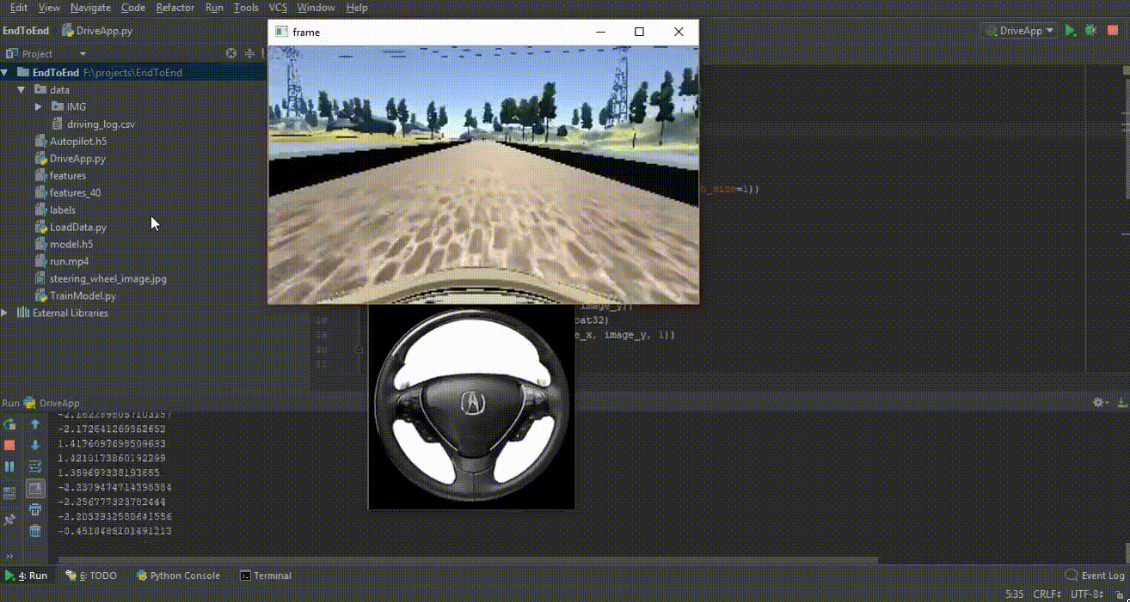
\includegraphics[width=.9\linewidth]{./img/project-running.png}
\caption{\label{fig:org58af00a}Testing model on simulator}
\end{figure}
Car owners who buy cars self driving hardware installed can choose software on their own.
Biggest issue in self-driving cars is safety, even though some people believe AI driven cars
will reduce accident rates drastically. Technology still fails to amuse us due to various
reasons. So our Virtual Simulation of Self Driving Car will not be just a program for self
driving but also it is a simulation which tests the program capabilities. Virtual simulation
will allow people around the world to create their own self-driving programs but also to test
it’s accuracy.
The benefits of fully autonomous vehicles can go way beyond removing the
need of a human driver. Transportation services such as Uber will start using selfdriving
cars instead of human drivers, and might become a cheaper and better
alternative for end consumers than owning a car. This will represent a shift on the
way cities are planned, as fewer parking places will be needed, and most importantly,
in a smart city with most of its vehicles being connected and autonomous,
traffic optimization will be able to be heavily applied by coordinating movement.
This will result in a major decrease on travel time, and it will also save lives as
emergency services will be able to reach their destinations faster.
\clearpage

\section{Literature review}
\label{sec:orgd5a5e2f}
\textbf{Self-Driving cars} have been said to be the next big disruptive innovation in the years to come.
Considered as being predominantly technology driven, it is supposed to have massive societal
impact in all kinds of fields. In this section a brief overview on the technology and development
will prove helpful to understand the need of customer acceptance.

In 2009, Google started research in self-driving cars privately.In 2010, major automobile
industries started research in autonomous vehicles. Audi first released and tested a driverless
car AudiTTS in the mountains. In 2011, General Motors also released an Electric Networked vehicle.
In 2012, Volkswagen created a temporary auto pilot (TAP) and tested in a highway at a speed of 130km/h.
In 2013 Toyota created semi-autonomous vehicles with sensors and communication systems.
In 2014, Mercedes S-class was released in market with many autonomous options in city and
highway traffic at a speed of up to 200MPH. Tesla Motor also created the first version of
Autopilot Model Swith semi-autonomous vehicles.

There is a growing interest in developing user interfaces of self-driving cars or automated
vehicles which are also known as driverless cars. The literature on Self-driving cars has
steadily been growing. However, there has not been any effort to systematically select,
review, and synthesize the literature on this topic. A systematic literature review is
conducted that reports different perspectives of autonomous cars like liabilities and
responsibilities of these Self-driving cars in case of accidents, ethics related to decision
making, potentials and drawbacks of using Self-driving cars, people's perspective about them
and challenges faced by them.
\clearpage

\section{Solution to the problem}
\label{sec:org83eb81b}
\subsection{Convolutional Neural Networks}
\label{sec:orgf01cacd}
Artificial Intelligence has been witnessing a monumental growth in bridging the gap between the capabilities
of humans and machines. Researchers and enthusiasts alike, work on numerous aspects of the field to make amazing
things happen. One of many such areas is the domain of Computer Vision.
\begin{figure}[htbp]
\centering
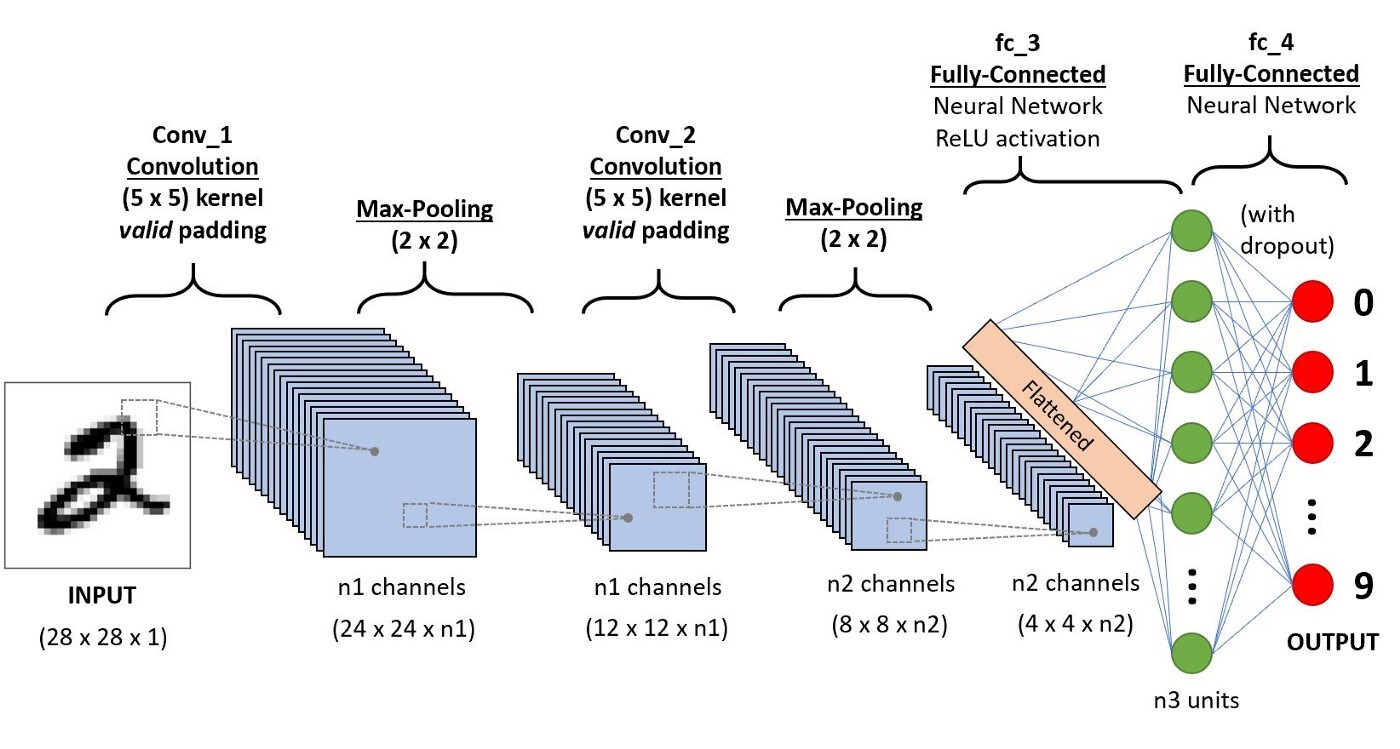
\includegraphics[width=.9\linewidth]{./img/cnn.jpg}
\caption{\label{fig:org4ccaa3d}A CNN sequence to classify handwritten digits}
\end{figure}
The agenda for this field is to enable machines to view the world as humans do, perceive it in a similar manner
and even use the knowledge for a multitude of tasks such as Image \& Video recognition, Image Analysis \&
Classification, Media Recreation, Recommendation Systems, Natural Language Processing, etc. The advancements in
Computer Vision with Deep Learning has been constructed and perfected with time, primarily over one particular
algorithm — a Convolutional Neural Network.
\clearpage

\section{Methodology}
\label{sec:org5279fea}
Software development methodology is a process or series of processes used in software development.
Again, quite broad but that it is things like a design phase, a development phase. It is ways of
thinking about things like waterfall being a non iterative kind of process. Generally it takes the
form of defined phases. It is designed to describe the how of the life cycle of a piece of software.
It is also codified communication. So you’re actually setting a set of norms between a group of people
that say this is how you’re going to work and this is how you’re going to pass information between
each of you in certain ways; whether that is documentation, whether that is discussion, whether that
is drawings on paper.
The method used for developing this system is \textbf{Agile} and \textbf{Lean}.
\subsection{Agile Methodology}
\label{sec:org26d740c}
To overcome the fast-changing organizational business needs using traditional methods,
agile methods were introduced. \textbf{Agile} methods aid in and focus on developing solutions
more quickly and efficiently. When you break it down to the core concepts, the \textbf{Agile}
development is not that difficult. And while it may seem wasteful with the number of
meetings involved, it saves a lot of time by optimizing the development tasks and
reducing the errors during the planning stages.
\begin{figure}[htbp]
\centering
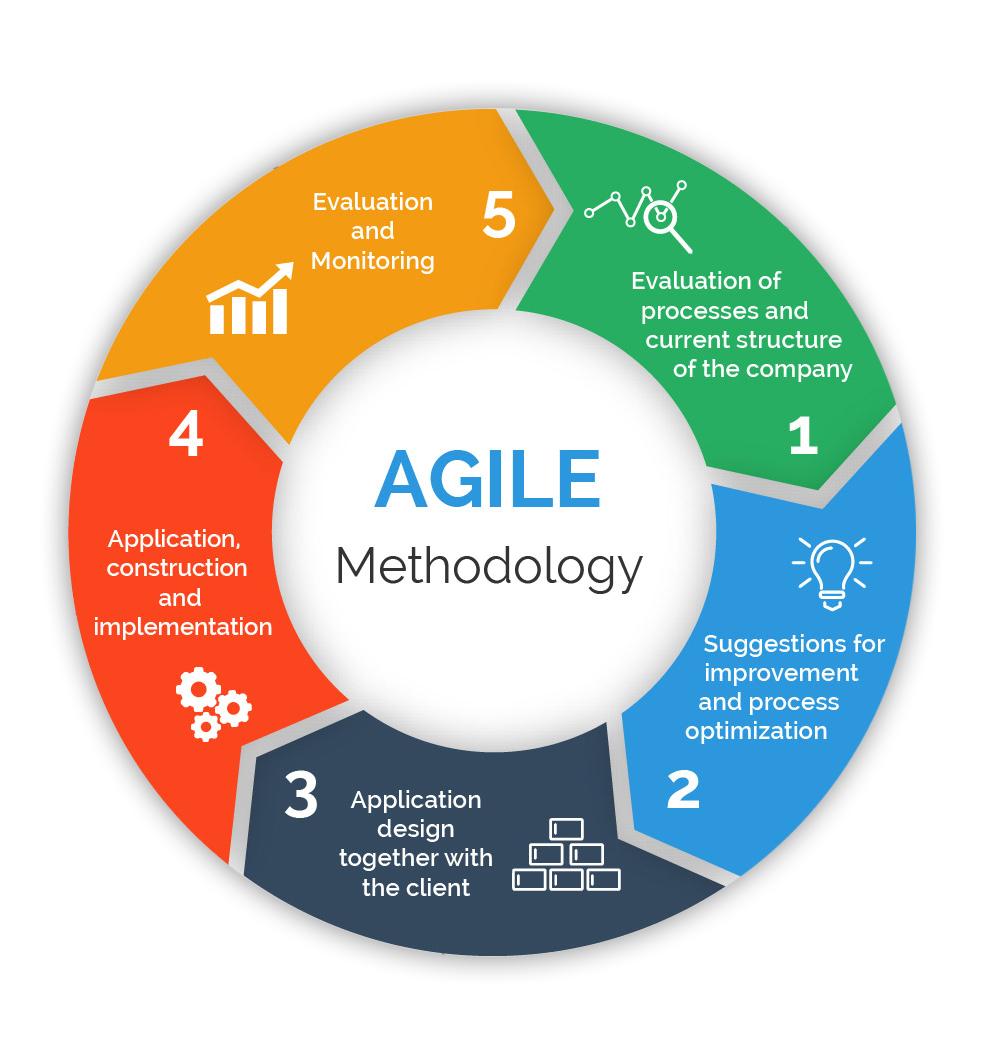
\includegraphics[width=.9\linewidth]{./img/agile.png}
\caption{\label{fig:org90c0f76}This is the caption for the next figure link (or table)}
\end{figure}
\clearpage

\section{Requirement specification}
\label{sec:org6972cfe}
To run a virtual simulation high end computer is needed and if we train the model of self driving car
we need a good GPU power to train the model. Considering the project will run on Unity game engine and
the self-driving car model was pre trained, the project itself only requires the recommended Unity
engine system requirement.
\subsection{System Requirements}
\label{sec:org9b9ff4b}
To use this tool efficiently, all computer software needs certain hardware components or
other software resources to be present on a computer. These prerequisites are known as system
requirements and are often used as a guideline as opposed to an absolute rule.
\begin{center}
\begin{tabular}{ll}
\hline
Operating System & Windows: 7 SP1+, 8, 10, 64-bit versions only.\\
 & macOS: 10.12+\\
 & Linux: Fixed at: Ubuntu 16.04, 18.04 and CentOS 7\\
\hline
CPU & SSE2 instruction set support\\
\hline
GPU & Graphics card with DX10 (shader model 4.0) capabilities\\
\hline
\end{tabular}
\end{center}
\subsection{Device Support}
\label{sec:org23a58ae}
Device support is the process of providing diagnostic, troubleshooting, maintenance
and repair services to a computer or similar device. It allows end users to seek and
receive specialized computer maintenance and management services, either locally from
their home/office or remotely via the Internet.
\begin{center}
\begin{tabular}{ll}
\hline
iOS & Mac computer running minimum\\
 & macOS 10.12.6 and Xcode 9.4 or higher\\
\hline
Android & Android SDK and Java Development Kit (JDK)\\
\hline
Universal Windows Platform & Windows 10 (64-bit), Visual Studio\\
 & 2015 with C++ Tools component or later\\
 & and Windows 10 SDK\\
\hline
\end{tabular}
\end{center}
\clearpage
\section{Build procedure}
\label{sec:orgcb2621c}
\clearpage
\section{Conclusion}
\label{sec:orgc73452d}
\clearpage
\section{Outcome Snapshots}
\label{sec:org5753b43}
\begin{figure}[htbp]
\centering
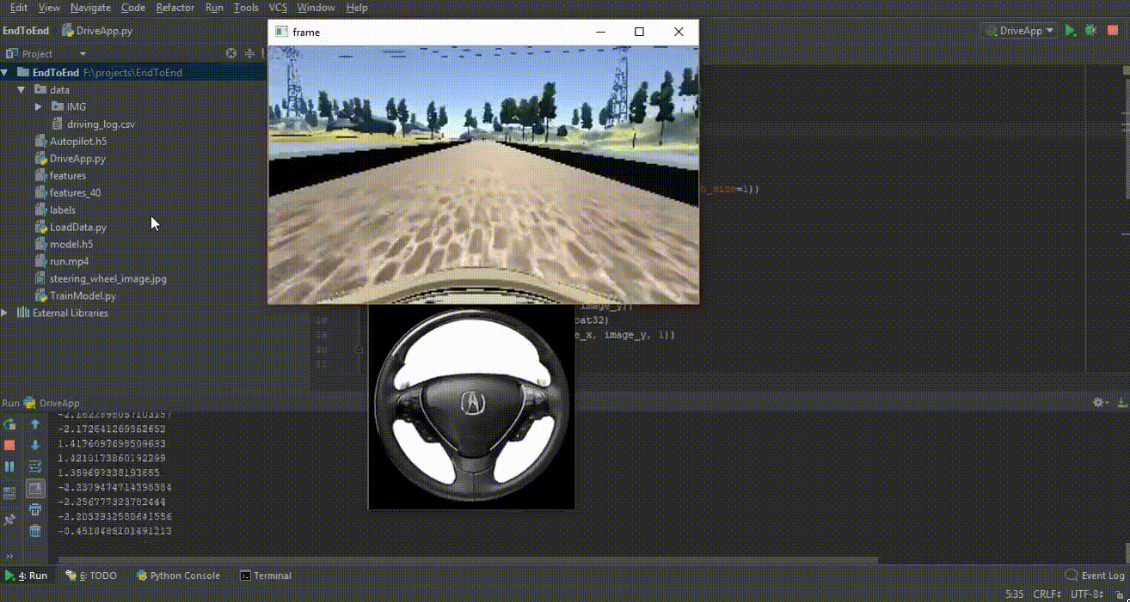
\includegraphics[width=.9\linewidth]{./img/project-running.png}
\caption{\label{fig:orga7b5b99}Testing model on simulator}
\end{figure}

\begin{figure}[htbp]
\centering
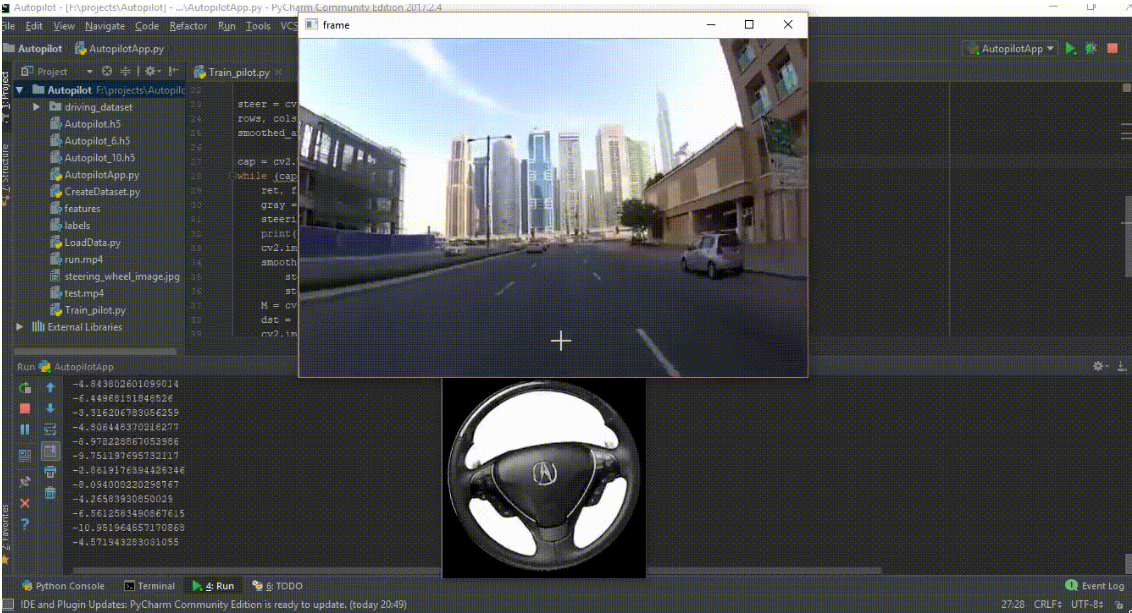
\includegraphics[width=.9\linewidth]{./img/project-running2.png}
\caption{\label{fig:orgfb4327a}Testing model on a driving video}
\end{figure}

\subsection{Directory structure}
\label{sec:orgca7652e}
\begin{verbatim}
├── Autopilot Parent (Current Directory)
    ├── Autopilot
	├── models 
	├── resources
	├── Trainer.py
	├── DataLoader.py
	└── Main Application.py
    ├── Autopilot_V2
	├── models 
	├── resources
	├── Trainer.py
	├── DataLoader.py
	└── Main Application.py
    ├── LICENSE
    ├── requirements.txt
    └── readme.md
\end{verbatim}

\clearpage
\section{Future enhancements}
\label{sec:orgb8e86d0}
\subsection{Emergency lane changes}
\label{sec:org5019f65}
Whether on highways or two-lane roads it may happen that an obstacle will
suddenly require a lane change, for example, when an animal crosses the road,
or when a landslide occurs. This sudden lane change may represent a dangerous
situation, as it is possible that the vehicles on the other lane are approaching from
behind in a much higher speed.
By broadcasting a sudden lane change event for the vehicles behind, they
will be able to reduce their speed faster, before they can visually detect the car
changing lanes, reducing the risk of an accident.
\subsection{Early obstacle avoidance}
\label{sec:org665a42f}
Obstacles such as boulders, broken vehicles, or road work can cause massive traffic
as they usually involve obstructing an entire lane. On roads without
closed lane signals, by broadcasting the detection of an obstacle on the lane, the
vehicles behind would be able to change lanes before reaching the obstacle, reducing traffic.
\subsection{Temporary stops}
\label{sec:org36105e6}
Cars and buses can stop to pickup/drop passengers for short periods of time.
As in the last example, this could also increase traffic. These vehicles could send
a notification that they will stop for a short period of time, allowing vehicles that are
approaching from behind to decide whether or not to change lanes based on their
location and on how much time the vehicle is going to be stopped.
\subsection{Junctions and Intersections}
\label{sec:orge4ad1b7}
There are many mathematical models for optimizing traffic in junctions and
intersections. These models could be optimized by making vehicles that are able
to coordinate their movement.
\subsection{Emergency vehicles}
\label{sec:orgcfd8698}
An emergency vehicle could broadcast its presence for vehicles ahead, so
that they could change lanes early to give priority to it. This will make
the emergency vehicles reach their destinations faster, something that could save lives.
\subsection{Pile-up avoidance}
\label{sec:org017c076}
In the unfortunate event of an accident, vehicles could broadcast a car crash
notification that will make vehicles approaching from behind reduce their speed,
decreasing the risk of a pile-up. Also, this will allow the other vehicles to reroute,
which may reduce the traffic generated by the accident
\clearpage
\section{Appendix A}
\label{sec:org1c7b215}
\subsection{Python environment setup}
\label{sec:org6b49827}
On terminal, inside the project file, run the following shell command to create the environment:
\begin{verbatim}
python -m venv env
source env/bin/activate
\end{verbatim}
\subsection{Installing \texttt{pip} requirements}
\label{sec:org32e1991}
\begin{verbatim}
pip install -r requirements.txt
\end{verbatim}
\clearpage
\section{Appendix B}
\label{sec:org93f1d1d}
\subsection{Contents of the CD}
\label{sec:org20cd80b}
The CD provided with this report contains the following data :
\subsubsection{Author's indentity}
\label{sec:org8065e87}
This is a text file (.txt) that contains each of the author’s details like Name, University,
Roll Number, E-mail ID, Course, Principle, Nationality, Current Address.
\subsubsection{Hardware Requirements}
\label{sec:org60f22df}
The hardware devices required for using the project smoothly and successfully.
\subsubsection{Software Requirements}
\label{sec:orgcb6ac65}
The software within the system required for using the project smoothly and successfully.
\subsubsection{Dependencies}
\label{sec:org21b44a6}
The piece of software that relies on other software.
\subsubsection{Software (project)}
\label{sec:org6d80969}
Entire project folder with all the code files and dependencies, modules, package, etc that can run.
\clearpage
\section{References}
\label{sec:org3ea9852}
\end{document}
